Ben Trout

2014-09-19

Brainstorming, Designing, and Promoting FTC

\begin{tabular}{|p{5cm}|p{5cm}|}
 \hline
 Brainstorming&
 We started our brainstorming by making three subsystems for scoring blocks:
 Intake, Lifter, and Scorer. We had a bunch of designs down and ideas flowing.
 As a team we we’re able to list pros and cons of all the designs mentioned and narrowed
 it down to just a few quality designs.
 \\
 \hline
 Designing&
 Once we had our ideas pinpointed that we thought would be best for accomplishing
 the challenge we started to design different components of the robot.
 Me, Nick, and Alex mainly focused on the intake method of picking up balls.
 \\
 \hline
 Promoting FTC and FIRST&
 I went to a lego robotics meeting with my FRC team for recruiting Lego Robotics coaches
 for the FLL league at liberty that we’re starting up. We wanted to promote all three
 levels of FIRST. We had old lego robots for demo, I brought a ball shooting FTC robot
 I built and my FRC team brought their worlds robot from last year.
 We demo’d all the robots and got the kids exited for robotics, hopefully they will
 move up in the FIRST levels and be on the Liberty FTC team in the future.
 \\
 \hline
\end{tabular}

\section*{Brainstorming}
Ways to play the game:
\begin{itemize}
 \item Tip rolling goal onto ramp. Shuttle balls up and down ramp
 \item Grab rolling goal and drive around with it putting balls in
 \item Put balls into center goal %TODO This may need to be corrected
\end{itemize}
Subsytems:
\begin{itemize}
 \item Intake
 \begin{itemize}
  \item scooper
  \item rotating brush
  \item suction
  \item rotating wheels
 \end{itemize}
 \item Lifter
\end{itemize}

Subsystems:
\begin{itemize}
 \item Intake
 \begin{itemize}
  \item scooper
  \item rotating brush
  \item conveyor belt
  \item suction
  \item rotating wheels
 \end{itemize}
 \item Lifter
 \begin{itemize}
  \item batched
  \item continuous feed
 \end{itemize}
 \item Scorer
 \begin{itemize}
  \item active dumper
  \item passive dumper
 \end{itemize}
 \item Goal attachment
 \begin{itemize}
  \item claw
 \end{itemize}
 \item Drive base
\end{itemize}

Lifter/Scorer:

Trio of Archimedes Screw

Conveyer belt Tri belt Pulley system

Guided launcher mechanism

Ball sorter

Scissor lift with conveyer belt to bring balls up

Spring Shot with guided tube

Pulley system

surgical tubing sling shot with guided tube

\section*{Designing}
As a team we finalized on rotating brushes to intake the balls,
a surgical tubing sling shot with a guided tube into the goals,
and a passive dumper. Our main idea for scoring is using claws to attach
to the base of the goal and carry it around with as we launch balls up a tube and
deflected into the goal. We have rotating brushes that intake the balls into a
slingshot that launches the balls into a guided tube that is extended and retracted by
a pulley system. The only part of our brainstorming that we have designed is our intake:

\begin{center}
 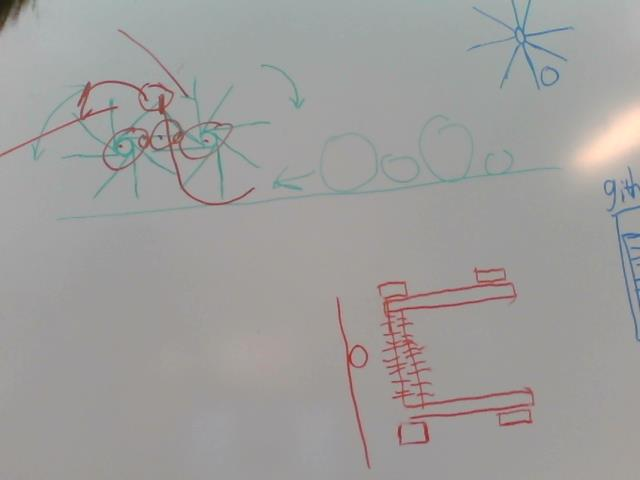
\includegraphics[width=10cm]{./Entries/Images/RotatingBrushes.jpg}
 \end{center}

The balls flow under our robot where one rotating brush brushes up a wall bring the
balls up into the robot and deflected onto a ramp that leads the balls into the
slingshot. The odds of surpassing the five ball limit is low so we aren’t going to incorporate a sensor yet. 
We did a lot of calculations like how many balls we’ll pick up per second, size of balls, and if different ideas like a scissor lift will fit in our Robot. I wasn’t in charge of calculating, but other team members like David and Matthew were.

\section*{Promoting FIRST}
At the meeting put on by my FRC team our main goal was to get Lego Robotics coaches for the starting lego robotics program at Liberty. We want to get young students excited for robotics and mainly Lego robotics. But we don’t want these kids robotics to end with FLL. We want to start their robotics program early and keep them going through the levels of FIRST so that when they get to FRC they are used to robotics and accustomed. The FRC team brought that robot and demo’d it and I brought a small FTC robot I made to demo for the kids. We had all three levels of FIRST robots present to get the kids and parents excited for Robotics.

\begin{center}
 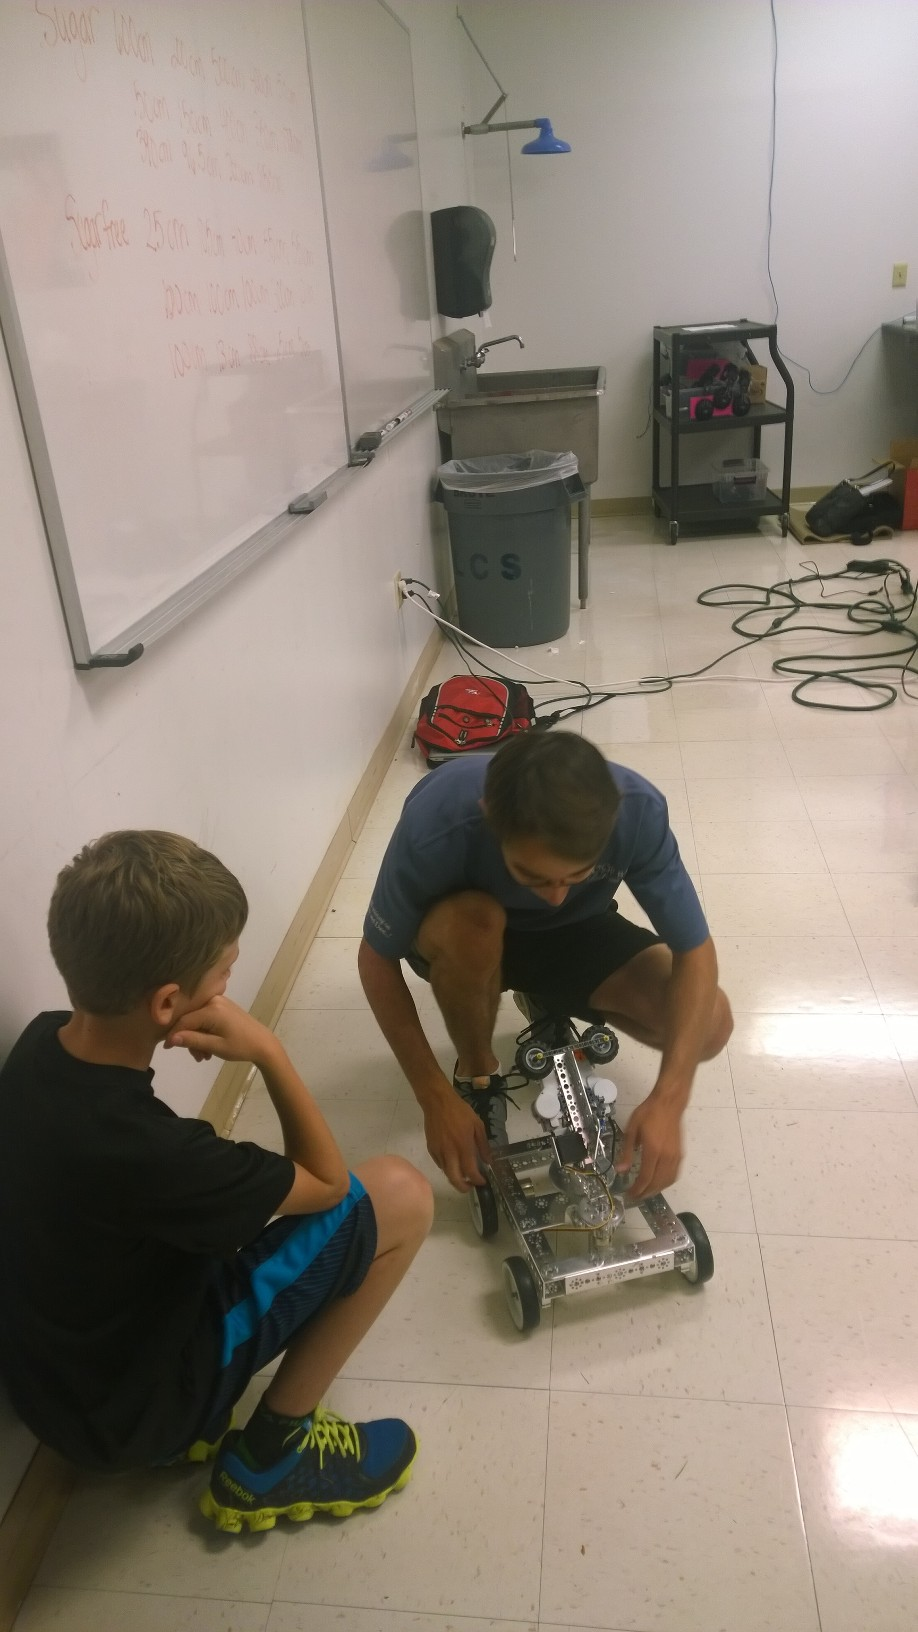
\includegraphics[width=10cm]{./Entries/Images/BenDemoingFTCRobottoAnFLLstudent.jpg}
 \end{center}
